\documentclass[11pt,a4paper]{article}

% Pacotes essenciais
\usepackage[utf8]{inputenc}
\usepackage[T1]{fontenc}
\usepackage{lmodern}
\usepackage[portuguese]{babel}
\usepackage{graphicx}
\usepackage{amsmath}
\usepackage{amsfonts}
\usepackage{amssymb}
\usepackage{float}
\usepackage{caption}
\usepackage{subcaption}
\usepackage{xcolor}
\usepackage{colortbl}
\usepackage{fancyhdr}
\usepackage{geometry}
\usepackage{titlesec}

\usepackage[hidelinks]{hyperref}
\usepackage[alf]{abntex2cite}
\usepackage{booktabs}
\usepackage{array}
\usepackage{pdflscape}

\usepackage{enumitem}
\usepackage{tikz}
\usepackage[most]{tcolorbox}


% Definição das cores
\definecolor{headercolor}{HTML}{b11116}
\definecolor{secondarycolor}{HTML}{3a5461}
\definecolor{primaryA}{HTML}{AED5FF}
\definecolor{primaryB}{HTML}{FFC2C2}

% Configuração da página
\geometry{
    a4paper,
    top=2.8cm,
    bottom=2.5cm,
    left=2.5cm,
    right=2.5cm,
    headheight=1.2cm,
    headsep=0.5cm
}

% Configuração do cabeçalho
\pagestyle{fancy}
\fancyhf{}
\renewcommand{\headrulewidth}{0pt}
\renewcommand{\footrulewidth}{0.5pt}

\fancyhead[L]{%
    \begin{tikzpicture}[remember picture, overlay]
        \fill[headercolor] (current page.north west) rectangle ([yshift=-1.2cm]current page.north east);
        \node[anchor=west, inner sep=0pt] at ([xshift=1cm, yshift=-0.6cm]current page.north west) 
            {\includegraphics[height=0.8cm]{imgs/base/fatec-rgt.png}};
        \node[anchor=east, inner sep=0pt] at ([xshift=-1cm, yshift=-0.6cm]current page.north east) 
            {\includegraphics[height=0.9cm]{imgs/base/cps-logo.png}};
        \node[anchor=east, inner sep=0pt] at ([xshift=-2.8cm, yshift=-0.6cm]current page.north east) 
            {\includegraphics[height=1.05cm]{imgs/base/governo-sp-secretaria-logo.png}};
    \end{tikzpicture}
}

\fancyfoot[L]{\footnotesize\textcolor{secondarycolor}{Faculdade de Tecnologia do Estado de São Paulo\\ fatecregistro.cps.sp.gov.br}}
\fancyfoot[R]{\thepage}

% Configuração dos títulos das seções
\titleformat{\section}
    {\normalfont\large\bfseries\color{secondarycolor}}
    {\thesection}{1em}{}

\titleformat{\subsection}
    {\normalfont\normalsize\bfseries\color{secondarycolor}}
    {\thesubsection}{1em}{}

\begin{document}

% ===== CAPA =====
\begin{titlepage}
    \centering
    
    \begin{tikzpicture}[remember picture, overlay]
        \fill[headercolor] (current page.north west) rectangle ([yshift=-1.2cm]current page.north east);
        \node[anchor=west, inner sep=0pt] at ([xshift=1cm, yshift=-0.6cm]current page.north west) 
            {\includegraphics[height=0.8cm]{imgs/base/fatec-rgt.png}};
        \node[anchor=east, inner sep=0pt] at ([xshift=-1cm, yshift=-0.6cm]current page.north east) 
            {\includegraphics[height=0.9cm]{imgs/base/cps-logo.png}};
        \node[anchor=east, inner sep=0pt] at ([xshift=-2.8cm, yshift=-0.6cm]current page.north east) 
            {\includegraphics[height=1.05cm]{imgs/base/governo-sp-secretaria-logo.png}};
    \end{tikzpicture}
    
    \vspace*{3.5cm}
    
    {\normalsize FACULDADE DE TECNOLOGIA DO ESTADO DE SÃO PAULO\par}
    \vspace{0.5cm}
    
    {\normalsize DESENVOLVIMENTO DE SOFTWARE MULTIPLATAFORMA\par}
    
    \vspace{4cm}
    
    {\normalsize ARTEFATOS DO PROJETO DE SOFTWARE\par}
    
    \vspace{0.3cm}
    
    {\normalsize Criação de Camarão em Cativeiro com Monitoramento IoT para Gastronomia\par}
    
    \vspace{3cm}
    
    {\normalsize
    Davi Mathais de Almeida\\
    Leandro Augusto De Souza Muniz\\
    Tiago de Lara Rodrigues
    }
    
    \vfill
    
    {\small Registro -- SP\\
    2026}
    
\end{titlepage}

\pagestyle{fancy}

% ===== SUMÁRIO =====
\tableofcontents
\newpage

\subsection*{Lista de Artefatos e suas Finalidades}

\begin{itemize}
    \item \textbf{CANVAS:} Modelo de negócio e estratégia
    \item \textbf{SWOT:} Análise estratégica de forças, fraquezas, oportunidades e ameaças
    \item \textbf{UX/UI:} Design de interface e experiência do usuário
    \item \textbf{Website:} Estrutura e especificações técnicas web
    \item \textbf{Diagramas UML:} Modelagem visual do sistema
    \item \textbf{DevOps:} Infraestrutura, automação e práticas de entrega contínua
\end{itemize}

\vspace{0.5cm}
\noindent\rule{\textwidth}{0.5pt}

\newpage

% ===== CANVAS =====
\section{CANVAS: Modelo de Negócio e Estratégia}

O Business Model Canvas é uma ferramenta visual estratégica que permite descrever, analisar e projetar modelos de negócio de forma clara e objetiva. O canvas é dividido em nove blocos fundamentais que cobrem as principais áreas de um negócio.

\begin{table}[H]
\centering
\caption{Business Model Canvas - Visão Geral}
\label{tab:canvas}
\small
\begin{tabular}{|>{\raggedright\arraybackslash}p{2.5cm}|>{\raggedright\arraybackslash}p{2.5cm}|>{\raggedright\arraybackslash}p{2.7cm}|>{\raggedright\arraybackslash}p{2.9cm}|>{\raggedright\arraybackslash}p{2.5cm}|}
\hline
\textbf{Parcerias Principais} & \textbf{Atividades Chave} & \textbf{Proposta de Valor} & \textbf{Relacionamento} & \textbf{Segmentos} \\
\hline
Fornecedores de sensores e microcontroladores (ESP32), provedores de infraestrutura em nuvem (Vercel, Render), consultores técnicos em carcinicultura & Coleta e interpretação de dados de temperatura, pH e amônia; geração de alertas em tempo real; manutenção da plataforma e dos sensores & Redução do tempo de manejo manual (de cerca de 5h/dia para monitoramento automatizado), alertas imediatos, maior precisão no controle da qualidade da água & Suporte técnico contínuo, treinamentos de uso, canal direto via chat/WhatsApp com a empresa & Pequenos e médios produtores de camarão e cooperativas de carcinicultura \\
\hline
 & \textbf{Recursos Principais} & & \textbf{Canais} & \\
\hline
 & Sensores (DS18B20, Ph4502, MQ-135), microcontrolador ESP32, plataforma web/PWA (React/Next.js, Node/Express, MongoDB Atlas), dispensador automatizado de ração & & Indicação por consultores e associações do setor, feiras e eventos de aquicultura, redes sociais e e-mail para captação, telefone/chat para suporte pós-venda & \\
\hline
\multicolumn{2}{|>{\raggedright\arraybackslash}p{5.4cm}|}{\textbf{Estrutura de Custos}} & \multicolumn{3}{>{\raggedright\arraybackslash}p{8.5cm}|}{\textbf{Fontes de Receita}} \\
\hline
\multicolumn{2}{|>{\raggedright\arraybackslash}p{5.4cm}|}{\textbf{Fixos:} desenvolvimento e manutenção do sistema, hospedagem em nuvem (Vercel/Render). \textbf{Variáveis:} equipamentos IoT por instalação, marketing e aquisição de clientes} & \multicolumn{3}{>{\raggedright\arraybackslash}p{8.5cm}|}{Assinatura mensal ou anual (SaaS), taxa de instalação do sistema físico, treinamentos avulsos} \\
\hline
\end{tabular}
\end{table}

\subsection{Análise do Modelo de Negócio}

A proposta de valor se apoia em resultados mensuráveis do próprio protótipo, como tempo de resposta a alertas imediata e precisão validada dos sensores, o que reduz o risco de a proposta soar genérica frente à concorrência. Ainda assim, o modelo depende de uma premissa não testada: que produtores tradicionalmente pouco digitalizados aceitem pagar recorrentemente (assinatura) por um serviço cuja alternativa (manejo manual) tem custo percebido como zero, já que é mão de obra própria. Essa é a principal tensão do Canvas e deveria ser endereçada com mais clareza, por exemplo, comparando o custo da mão de obra desviada para outras tarefas com o valor da assinatura.

A separação entre parcerias e segmentos evita um erro comum: tratar o próprio cliente (produtor de camarão) como parceiro estratégico. Os parceiros reais são quem viabiliza a operação sem ser quem paga: fornecedores de hardware e provedores de nuvem, dos quais o negócio depende diretamente para funcionar, e consultores técnicos, que também aparecem como canal de aquisição por indicação, conectando os blocos de parceria e canal de forma coerente.

A estrutura de custos evidencia um ponto de atenção para a sustentabilidade do modelo de assinatura: os custos variáveis por instalação (sensores, microcontrolador) são custos únicos, mas o modelo de receita é recorrente, ou seja, a margem depende de reter o cliente por tempo suficiente para diluir o custo do hardware inicial, o que reforça a importância do bloco de relacionamento (suporte e treinamento) como mecanismo de retenção, não apenas de satisfação.

% ===== SWOT =====
\section{SWOT: Análise Estratégica}

A Análise SWOT (\textit{Strengths, Weaknesses, Opportunities, Threats}), ou FOFA (Forças, Oportunidades, Fraquezas e Ameaças) \cite{chiavenato2020}, é uma ferramenta de planejamento estratégico que identifica os fatores internos (forças e fraquezas) e externos (oportunidades e ameaças) que impactam o projeto.

\begin{table}[H]
\centering
\caption{Análise SWOT do Projeto}
\label{tab:swot}
\begin{tabular}{|p{7.2cm}|p{7.2cm}|}
\hline
\multicolumn{2}{|c|}{\cellcolor{secondarycolor!20}\textbf{FATORES INTERNOS}} \\
\hline
\textbf{FORÇAS (Strengths)} & \textbf{FRAQUEZAS (Weaknesses)} \\
\hline
\begin{minipage}[t]{7cm}
\begin{itemize}
    \item Sistema integrado que reúne monitoramento da água, alertas e programação remota da alimentação em uma única plataforma
    \item Alertas gerados a cada leitura recebida (leituras a cada minuto), por notificação \textit{push} e e-mail
    \item Aplicação web progressiva, acessível por celular e computador sem lojas de aplicativos, com perfis de acesso (proprietário e funcionários)
    \item Arquitetura baseada em componentes comerciais acessíveis (ESP32 e sensores de uso geral)
    \item Desenvolvimento orientado por relatos de produtores sobre perdas por falha de alimentação e por alteração dos parâmetros da água
\end{itemize}
\end{minipage}
&
\begin{minipage}[t]{7cm}
\begin{itemize}
    \item Monitoramento de amônia não validado: o sensor utilizado detecta gás no ar, e não amônia dissolvida
    \item Dependência de Wi-Fi e da API: o firmware não armazena leituras durante quedas de conexão
    \item Validação restrita a um aquário, uma espécie e cerca de 5,5 horas, sem validação com produtor ou cliente pagante
    \item Desvio sistemático no pH, com ajuste em ponto único e referência de baixo custo
    \item Dependência de componentes importados (ESP32, sensores), sujeitos a variação cambial e prazo de importação
\end{itemize}
\end{minipage}
\\
\hline
\multicolumn{2}{|c|}{\cellcolor{secondarycolor!20}\textbf{FATORES EXTERNOS}} \\
\hline
\textbf{OPORTUNIDADES (Opportunities)} & \textbf{AMEAÇAS (Threats)} \\
\hline
\begin{minipage}[t]{7cm}
\begin{itemize}
    \item Crescimento do mercado de aquicultura e da demanda por rastreabilidade/sustentabilidade na produção
    \item Parcerias com instituições de pesquisa (ex: universidades) para validação científica e captação de fomento
    \item Expansão do sistema para outros tipos de monitoramento ambiental agrícola
    \item Linhas de crédito e programas de incentivo à automação rural
\end{itemize}
\end{minipage}
&
\begin{minipage}[t]{7cm}
\begin{itemize}
    \item Cobertura \textit{Wi-Fi} limitada em propriedades rurais do Vale do Ribeira, exigindo soluções de conectividade alternativas
    \item Surtos de doenças no cultivo (ex: mancha branca), que afetam a demanda por qualquer tecnologia de manejo, independente de sua eficácia
    \item Volatilidade do preço do camarão no mercado, reduzindo a margem do produtor para investir em novas tecnologias
    \item Entrada de concorrentes com soluções similares e maior capital para escala comercial
\end{itemize}
\end{minipage}
\\
\hline
\end{tabular}
\end{table}

\subsection{Recomendações Estratégicas}

Com base na análise SWOT, as principais estratégias devem focar em:
\begin{itemize}
    \item \textbf{Forças + Oportunidades:} Utilizar os resultados validados (tempo de resposta, precisão dos sensores) como diferencial competitivo em parcerias com instituições de pesquisa, fortalecendo a credibilidade técnica do produto frente a linhas de fomento e programas de incentivo à automação rural
    \item \textbf{Forças + Ameaças:} Aproveitar a arquitetura de componentes acessíveis e a aplicação web sem lojas de aplicativos para reduzir a barreira de entrada de produtores de menor capital e, para mitigar a limitação de conectividade, priorizar o armazenamento local de leituras no ESP32 e investigar conectividade LoRa/4G
    \item \textbf{Fraquezas + Oportunidades:} Buscar validação com cliente real via parceria com instituição de pesquisa ou programa de incentivo, transformando o piloto acadêmico em piloto comercial monitorado, o que também endereça a falta de dados de mercado
    \item \textbf{Fraquezas + Ameaças:} Implementar plano de manutenção preventiva dos sensores e redundância na integração de hardware para reduzir o risco de falhas técnicas, especialmente relevante diante da entrada de concorrentes com maior capital, falhas recorrentes seriam o motivo mais fácil de perder espaço de mercado
\end{itemize}

\begin{table}[H]
\centering
\caption{Paleta de Cores do Projeto}
\label{tab:cores}
\begin{tabular}{|l|c|l|l|}
\hline
\textbf{Elemento} & \textbf{Cor} & \textbf{Código HEX} & \textbf{Uso} \\
\hline
Primária & \colorbox[HTML]{146AC7}{\phantom{AAA}} & \#146AC7 & Botões principais, links e destaques \\
Secundária & \colorbox[HTML]{FFC2C2}{\phantom{AAA}} & \#FFC2C2 & Identidade visual e destaques \\
Fundo & \fcolorbox[HTML]{BBBBBB}{FFFFFF}{\phantom{AAA}} & \#FFFFFF & \textit{Background} padrão \\
Fundo Informações & \fcolorbox[HTML]{BBBBBB}{F8FAFC}{\phantom{AAA}} & \#F8FAFC & \textit{Background} de informações \\
Texto & \colorbox[HTML]{000000}{\phantom{AAA}} & \#000000 & Texto principal \\
Sucesso & \colorbox[HTML]{166534}{\phantom{AAA}} & \#166534 & Mensagens de sucesso \\
Erro & \colorbox[HTML]{991B1B}{\phantom{AAA}} & \#991B1B & Mensagens de erro \\
\hline
\end{tabular}
\end{table}

O azul primário apresenta contraste de cerca de 5,4:1 com o branco, e as cores de sucesso e de erro superam 7:1, acima do mínimo de 4,5:1 recomendado pela WCAG para texto.

\begin{table}[H]
\centering
\caption{Tipografia do Projeto}
\label{tab:tipografia}
\begin{tabular}{|l|l|l|l|}
\hline
\textbf{Elemento} & \textbf{Fonte} & \textbf{Tamanho} & \textbf{Uso} \\
\hline
Títulos & Poppins Bold & 19--28 px & Cabeçalhos de seções e páginas \\
Corpo & Poppins Regular/Medium & 13--16 px & Texto principal e descrições \\
Botões & Poppins Medium & 13--14 px & Botões de ação e navegação \\
\hline
\end{tabular}
\end{table}

% ===== WEBSITE =====
\section{Website: Estrutura e Especificações Técnicas Web}

Esta seção documenta o website institucional/portfólio da equipe que desenvolveu a aplicação. O site da equipe serve para apresentar os membros, projetos realizados, competências e informações de contato.

\subsection{Mapa do Site da Equipe}

O mapa do site (\textit{sitemap}) mostra a hierarquia e organização das páginas do website da equipe:

\begin{figure}[H]
\centering
\resizebox{\linewidth}{!}{%
\begin{tikzpicture}[
    level 1/.style={sibling distance=4.5cm, level distance=1.5cm},
    level 2/.style={sibling distance=2.2cm, level distance=1.5cm},
    every node/.style={rectangle, draw, rounded corners, 
                       fill=secondarycolor!20, 
                       text width=2.1cm, 
                       align=center,
                       font=\small}
]
\node {Home}
    child {node {Sobre}
        child {node {Valores}}
        child {node {Objetivos}}
    }
    child {node {Serviços}
        child {node {Pitch}}
        child {node {Apresentação}}
    }
    child {node {Equipe}
        child {node {Membros}}
        child {node {Funções}}
    }
    child {node {Contato}
        child {node {Canais}}
        child {node {Formulário}}
    };
\end{tikzpicture}%
}
\caption{Estrutura de navegação do website da equipe}
\label{fig:sitemap}
\end{figure}

\subsection{Conteúdo das Páginas}

\textbf{Páginas principais do site da equipe:}

\begin{itemize}
    \item \textbf{Home:} Apresentação inicial da equipe
    \item \textbf{Sobre:} Conteúdo sobre nossos valores, missão e visão
    \item \textbf{Serviços:} Descrição dos serviços oferecidos pela equipe
    \item \textbf{Equipe:} Perfil dos membros (nome, foto, função, LinkedIn/GitHub)
    \item \textbf{Contato:} Formulário de contato e links para redes sociais
\end{itemize}

\subsection{Especificações Técnicas do Site da Equipe}

\begin{table}[H]
\centering
\caption{Stack Tecnológica do Website da Equipe}
\label{tab:stack-web}
\begin{tabular}{|l|l|>{\raggedright\arraybackslash}p{6cm}|}
\hline
\textbf{Camada} & \textbf{Tecnologia} & \textbf{Descrição} \\
\hline
Frontend & React 18 & Biblioteca JavaScript para interfaces \\
Build Tool e Bundler & Vite & Ferramenta de build de altíssima performance e dev server \\
Linguagem & TypeScript & Superset do JavaScript que garante tipagem estática segura \\
Estilização e Design & Tailwind CSS v4 & Framework CSS utilitário para responsividade e temas \\
Motor de Animações & Framer Motion & Biblioteca declarativa para animações e transições complexas \\
Iconografia Vetorial & Lucide / React Icons & Bibliotecas de ícones modernos, responsivos e otimizados \\
Serviço de Mensageria & EmailJS & Plataforma \textit{backend-as-a-service} para envio de e-mails \\
Hospedagem e \textit{Deploy} & Vercel & Plataforma de \textit{Edge Network} e \textit{hosting} com \textit{deploy} contínuo \\
\hline
\end{tabular}
\end{table}

% ===== DIAGRAMAS UML =====
\section{Diagramas UML: Modelagem Visual do Sistema}

A Unified Modeling Language (UML) \cite{booch2005} é uma linguagem de modelagem visual usada para especificar, visualizar, construir e documentar artefatos de sistemas de \textit{software}.

\subsection{Diagrama de Casos de Uso}

O diagrama identifica quatro atores principais e suas interações com o sistema: o Equipamento IoT, o Funcionário, o Dono e a Equipe técnica, cada um com permissões e funcionalidades específicas.

\begin{figure}[H]
    \centering
    \caption{Diagrama de Casos de Uso}
    \label{fig:diagrama-caso-uso}
        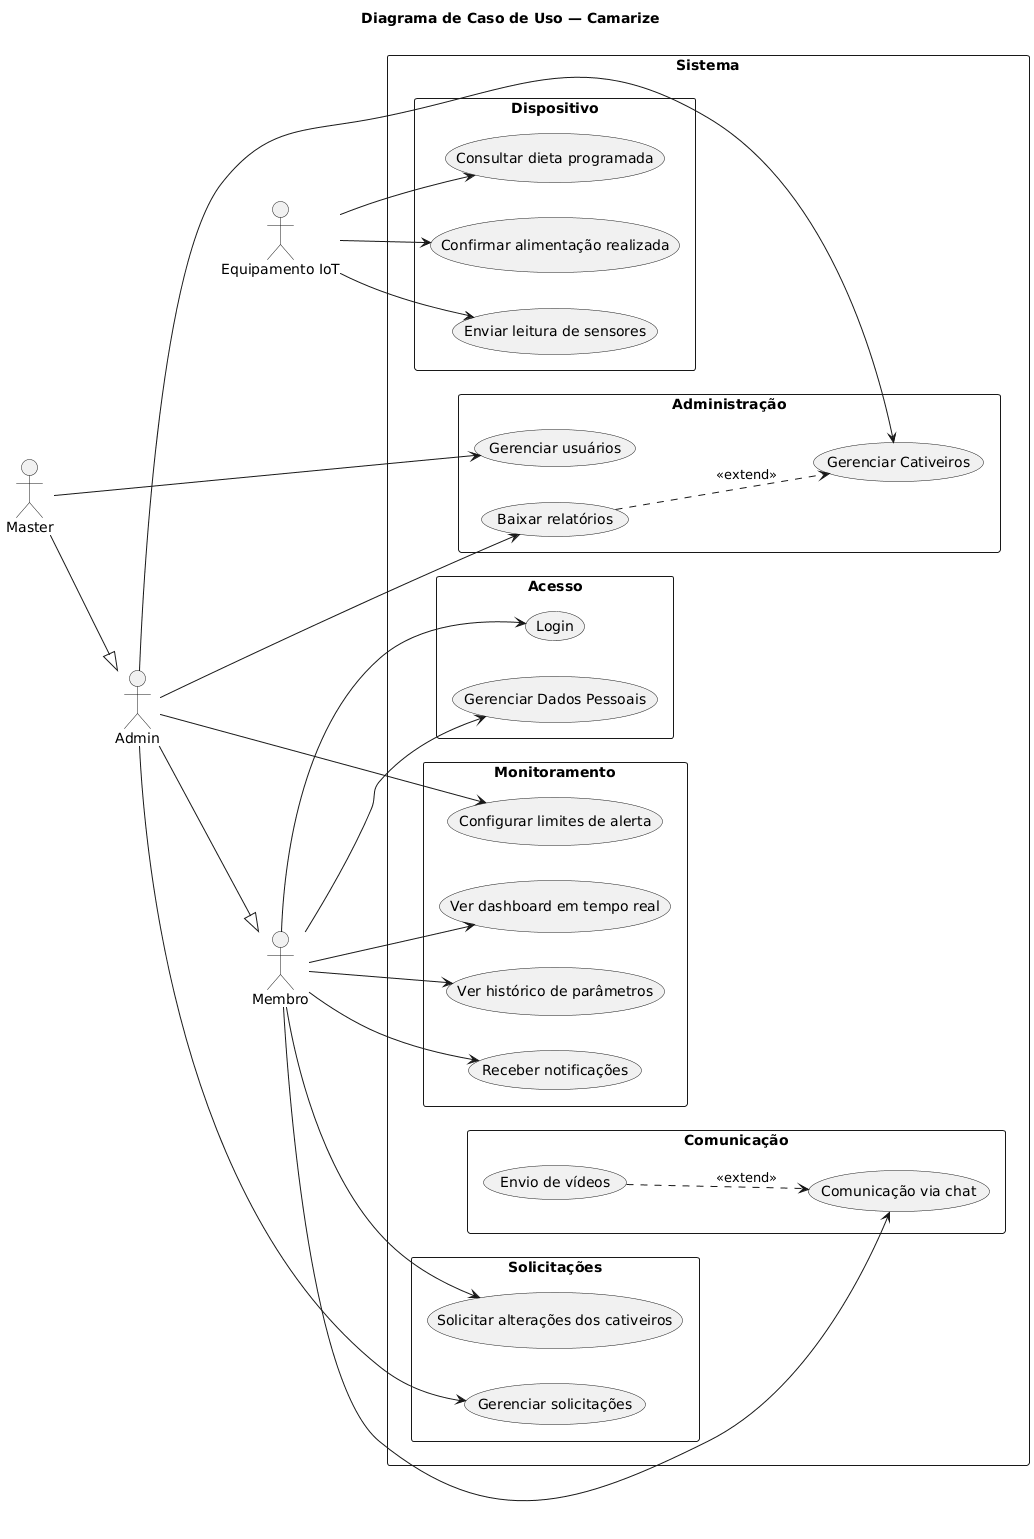
\includegraphics[width=0.8\textwidth]{imgs/diagrama_caso_uso.png}
    \\{\small Fonte: Autoria própria}
\end{figure}

\subsection{Diagrama de Classes}

Apresenta a estrutura orientada a objetos do sistema, com Users como classe central e seus relacionamentos com Cativeiros, Fazendas e os módulos de comunicação e notificações. Inclui os métodos de cada classe e as associações N:N por meio de coleções intermediárias.

\begin{figure}[H]
    \centering
    \caption{Diagrama de Classes}
    \label{fig:diagrama-classes}
        \makebox[\textwidth][c]{\includegraphics[width=1.1\textwidth]{imgs/diagrama_classes2.png}}
    \\{\small Fonte: Autoria própria}
\end{figure}
\newpage

\subsection{Diagrama de Objetos}

O diagrama de objetos ilustra instâncias concretas das classes do sistema em um cenário de uso, exemplificando os valores dos atributos e os vínculos entre objetos em tempo de execução.

\begin{figure}[H]
    \centering
    \caption{Diagrama de Objetos}
    \label{fig:diagrama-objetos}
        \includegraphics[width=1.0\textwidth]{imgs/diagrama_objetos.jpeg}
    \\{\small Fonte: Autoria própria}
\end{figure}

\subsection{Diagrama de Sequência}

Detalha três fluxos principais de interação: monitoramento em tempo real, visualização pelo usuário e controle de alimentação, envolvendo o Aplicativo, a API, o Banco de Dados e o ESP32.

\begin{figure}[H]
    \centering
    \caption{Diagrama de Sequência}
    \label{fig:diagrama-sequencia}
        \includegraphics[width=\textwidth]{imgs/diagrama_sequencia.png}
    \\{\small Fonte: Autoria própria}
\end{figure}

\subsection{Diagrama de Atividades}

Descreve o fluxo completo de operação do sistema, desde o cadastro do usuário até o ciclo contínuo de monitoramento e controle de alimentação, incluindo a lógica de verificação de limites e envio de alertas.

\begin{figure}[H]
    \centering
    \caption{Diagrama de Atividades}
    \label{fig:diagrama-atividades}
        \includegraphics[width=0.4\textwidth]{imgs/diagrama_atividades.png}
    \\{\small Fonte: Autoria própria}
\end{figure}

\subsection{Diagrama de Componentes}

Organiza o sistema em três blocos principais: Frontend (Next.js/Vercel), Backend (Node.js + Express/Render) e Componente IoT (ESP32), com comunicação via HTTPS e conexão ao MongoDB Atlas via Mongoose.

\begin{figure}[H]
    \centering
    \caption{Diagrama de Componentes}
    \label{fig:diagrama-componentes}
        \includegraphics[width=\textwidth]{imgs/diagrama_componentes.png}
    \\{\small Fonte: Autoria própria}
\end{figure}

\section{Infraestrutura de Rede}

A Figura~\ref{fig:rede} apresenta a infraestrutura de rede do sistema. No cativeiro, cada ESP32 DevKit V1, ao qual estão conectados os sensores de temperatura (DS18B20), pH (PH-4502C) e gases (MQ-135) e o motor de passo do dispensador de ração (28BYJ-48 com driver ULN2003), conecta-se por \textit{Wi-Fi} (padrão 802.11 b/g/n, banda de 2,4 GHz) a um roteador local, que dá acesso à internet por meio do provedor. A cada minuto, o ESP32 envia as leituras à API, hospedada na Render, e, nos horários programados, consulta a ela a configuração de alimentação, ambas as comunicações por HTTPS (porta 443).

A API grava os dados no MongoDB Atlas, banco de dados em nuvem, por conexão com TLS, e avalia cada leitura ao recebê-la. Quando um limite configurado é ultrapassado, ela aciona os alertas por e-mail (Nodemailer, via SMTP do Gmail) e por notificação \textit{push} (Web Push, protocolo VAPID). O frontend, desenvolvido em Next.js e disponibilizado como aplicação web progressiva, é hospedado na Vercel e acessado pelos usuários, em smartphone ou notebook, por HTTPS (porta 443), a partir de qualquer rede.

Como consequência dessa arquitetura, o funcionamento do sistema no cativeiro depende de conectividade \textit{Wi-Fi} local e de acesso à internet: durante interrupções, as leituras não são enviadas e o ESP32 não consegue consultar a configuração de alimentação.

\begin{figure}[H]
\centering
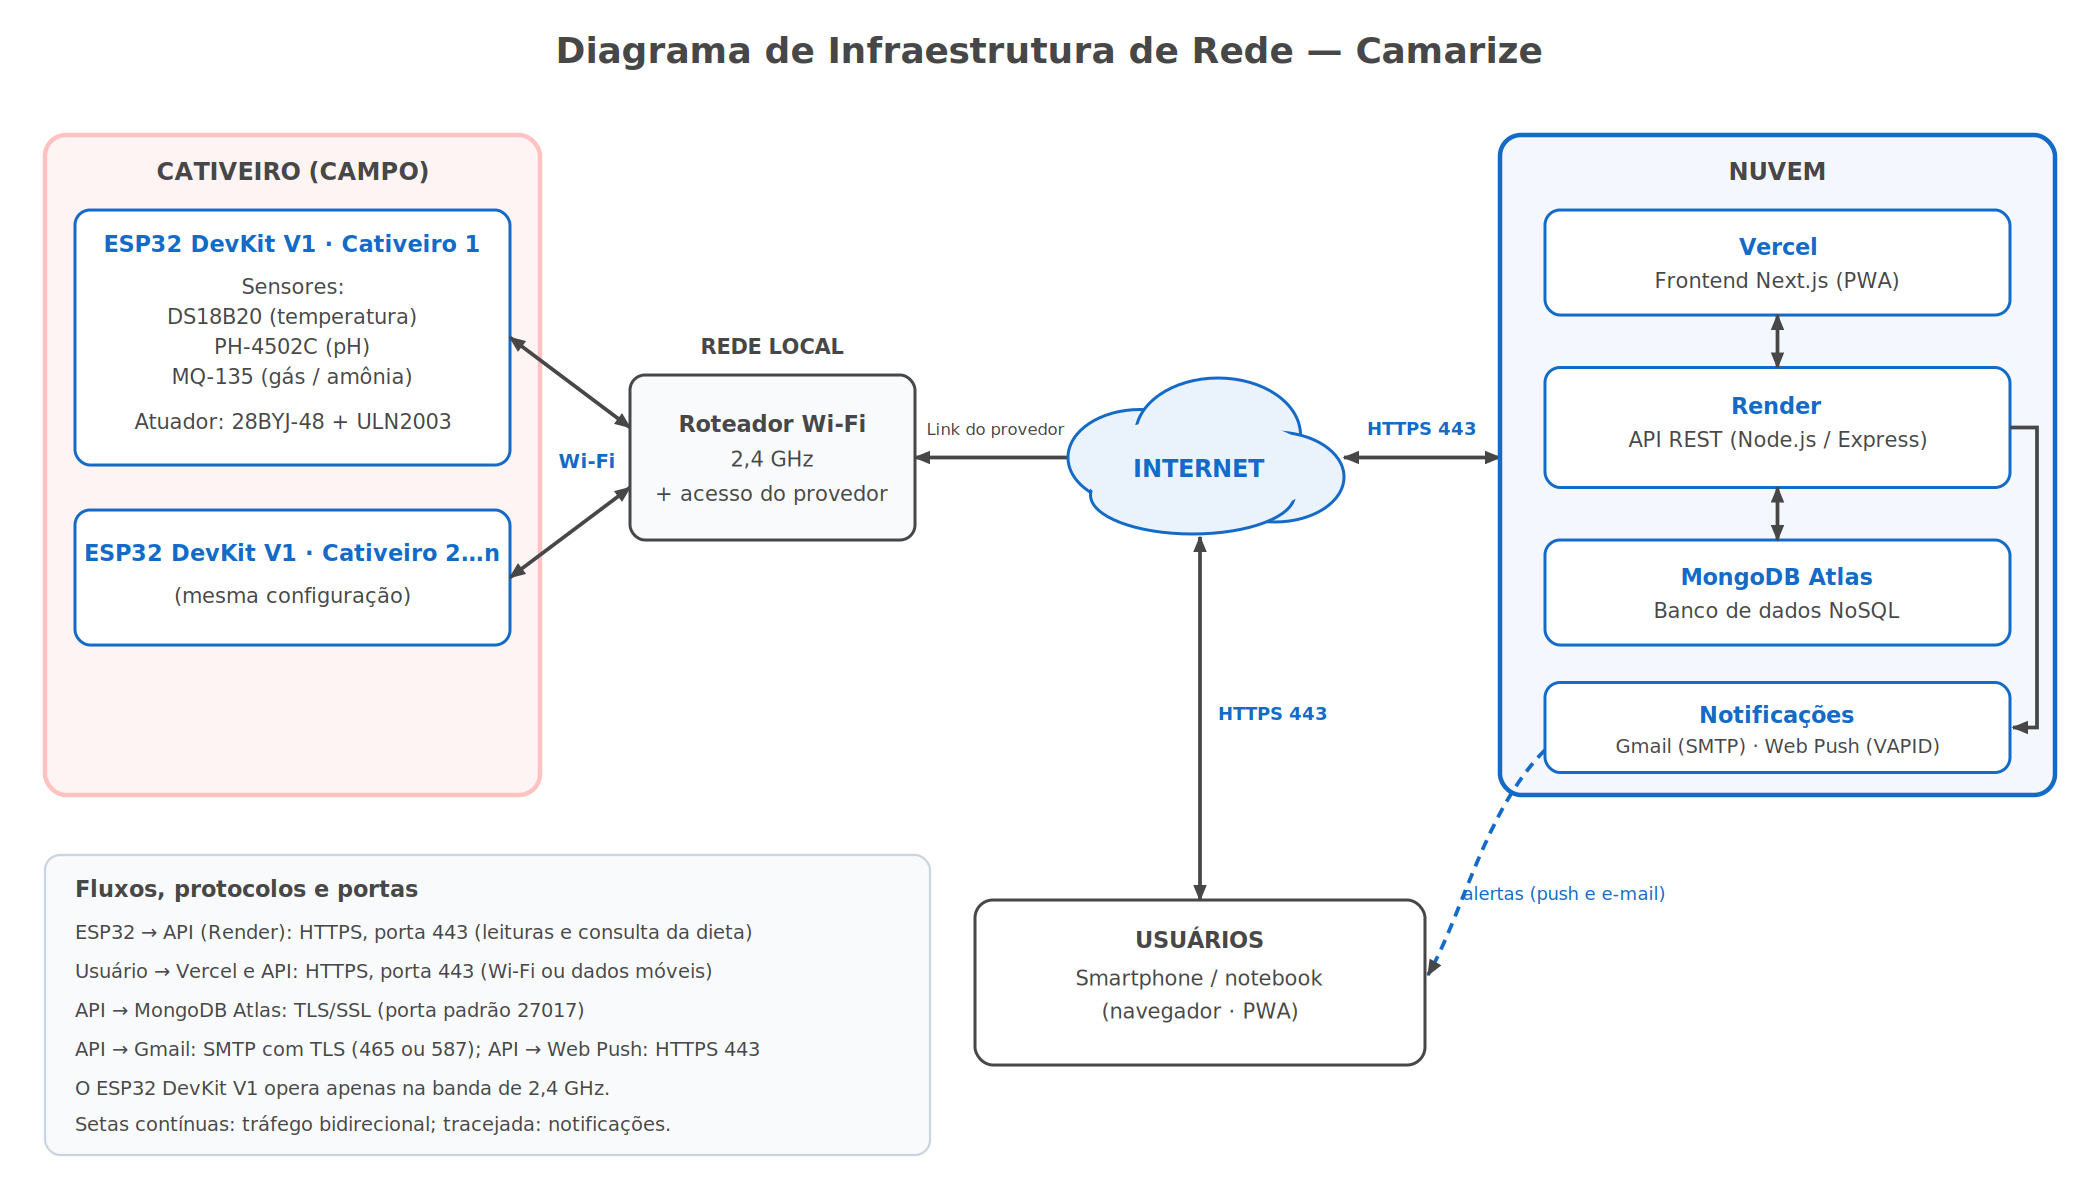
\includegraphics[width=1.0\linewidth]{imgs/diagrama_rede_camarize.png}
\caption{Diagrama de infraestrutura de rede do sistema}
\label{fig:rede}
\end{figure}

\subsection{Diagrama de Implantação}

Apresenta a distribuição física dos componentes em produção, incluindo a aplicação PWA na Vercel, a API REST no Render, o banco MongoDB Atlas e o ESP32 no ambiente do cativeiro, com \textit{deploy} contínuo via GitHub.

\begin{figure}[H]
    \centering
    \caption{Diagrama de Implantação}
    \label{fig:diagrama-implantacao}
        \includegraphics[width=0.8\textwidth]{imgs/diagrama_implantacao.png}
    \\{\small Fonte: Autoria própria}
\end{figure}

\subsection{Diagrama de Estados}

Modela o ciclo de vida de um cativeiro em quatro estados: AguardandoInstalação, Monitorando, EmAlerta e Inativo, com transições acionadas por eventos do sistema e ações do usuário.

\begin{figure}[H]
    \centering
    \caption{Diagrama de Estados}
    \label{fig:diagrama-estados}
        \includegraphics[width=0.8\textwidth]{imgs/diagrama_estados.png}
    \\{\small Fonte: Autoria própria}
\end{figure}

Para realizar a montagem dos diagramas, foi utilizada a ferramenta \textit{online} PlantUML, que permite a criação de diagramas UML através de código.

\section{Diagrama de Banco de Dados}

O diagrama de banco de dados representa a estrutura do banco de dados não relacional (NoSQL) utilizado no projeto, mostrando as coleções, seus campos e os relacionamentos entre elas.

\subsection{Modelo Conceitual}

O modelo conceitual representa as entidades e seus relacionamentos em alto nível, destacando as cardinalidades (1,1) e (1,N) entre todas as entidades do sistema de forma independente de tecnologia.

\begin{figure}[H]
    \centering
    \caption{Modelo Conceitual do Banco de Dados}
    \label{fig:modelo-conceitual}
        \makebox[\textwidth][c]{\includegraphics[width=1.1\textwidth]{imgs/modelo_conceitual.png}}
    \\{\small Fonte: Autoria própria}
\end{figure}

\subsection{Modelo Lógico}

O modelo lógico refina o conceitual para um esquema de coleções MongoDB, detalhando os documentos como Tipos\_camarao, Cativeiros, Sitios, Parametros\_atuais, Dietas, Sensores, Usuarios, entre outros, com seus campos, tipos de dados e referências entre coleções.

\begin{figure}[H]
    \centering
    \caption{Modelo Lógico do Banco de Dados}
    \label{fig:modelo-logico}
        \makebox[\textwidth][c]{\includegraphics[width=1.1\textwidth]{imgs/modelo_logico.jpeg}}
    \\{\small Fonte: Autoria própria}
\end{figure}

\subsection{Modelo Físico}

O modelo físico é a implementação final utilizando \textit{Mongoose Schemas}, com definições de tipos (String, Number, Boolean, Buffer, Map) e restrições (\texttt{required: true}), voltado para a criação direta das coleções no MongoDB Atlas, contemplando todas as entidades do sistema incluindo EmailSettings, PushSubscription, Conversation, Message e Request.

\begin{figure}[H]
    \centering
    \caption{Modelo Físico do Banco de Dados}
    \label{fig:modelo-fisico}
        \makebox[\textwidth][c]{\includegraphics[width=1.1\textwidth]{imgs/modelo_fisico.jpg}}
    \\{\small Fonte: Autoria própria}
\end{figure}

% ===== DEVOPS =====
\section{DevOps: Infraestrutura, Automação e Entrega Contínua}
DevOps \cite{kim2018} é uma cultura e conjunto de práticas que integra desenvolvimento de software (Dev) e operações de TI (Ops), focando em automação, colaboração e entrega contínua.

\subsection{Pipeline CI/CD}
O pipeline (GitHub Actions) é executado a cada \textit{push} e \textit{pull request} na branch \texttt{main} e reúne: lint (ESLint) e verificação de sintaxe da API; testes unitários da API com cobertura, executados contra um MongoDB em contêiner; \textit{build} de produção do frontend; verificação de segredos versionados; testes de ponta a ponta (Playwright); auditoria de dependências (\textit{npm audit}); e \textit{build} das imagens Docker. O job \texttt{ci-passed} consolida o resultado e, em \textit{push} na \texttt{main}, somente quando ele é bem-sucedido, os jobs de deploy publicam o frontend na Vercel (via CLI) e a API no Render (via API da plataforma, com verificação de prontidão). O auto-deploy nativo das duas plataformas foi desativado para que nada seja publicado sem passar pelo CI. Há ainda um fluxo de publicação manual, com confirmação explícita, para republicar um commit específico.

\begin{figure}[H]
\centering
\begin{tikzpicture}[
    node distance=3.3cm,
    every node/.style={rectangle, draw, rounded corners,
                       fill=secondarycolor!20,
                       text width=2.4cm,
                       align=center,
                       font=\footnotesize,
                       minimum height=1.4cm}
]
\node (push) {\textit{Push} ou \textit{pull request}\\na \texttt{main}};
\node (ci) [right of=push] {CI: lint, testes, \textit{build}, E2E, segredos, auditoria e Docker};
\node (gate) [right of=ci] {\texttt{ci-passed}\\(portão de qualidade)};
\node (deploy) [right of=gate] {Deploy\\Vercel e Render};
\node (manual) [below of=deploy, node distance=2cm, dashed] {Publicação manual\\(confirmação)};
\draw[->, thick] (push) -- (ci);
\draw[->, thick] (ci) -- (gate);
\draw[->, thick] (gate) -- (deploy);
\draw[->, thick, dashed] (manual) -- (deploy);
\end{tikzpicture}
\caption{Pipeline CI/CD}
\label{fig:cicd}
\end{figure}

\subsection{Configuração CI/CD}
O deploy depende do resultado do job \texttt{ci-passed}, que só reprova quando falham o lint, os testes da API, o \textit{build} do frontend, a verificação de segredos ou os testes de ponta a ponta; a auditoria de dependências e o \textit{build} das imagens Docker são informativos. O trecho a seguir (de \texttt{.github/workflows/ci.yml}) mostra a condição de publicação:

\begin{verbatim}
name: CI

on:
  push:
    branches: [main]
  pull_request:
    branches: [main]

concurrency:
  group: ci-${{ github.ref }}
  cancel-in-progress: true

jobs:
  lint-api:
    name: Lint API
    runs-on: ubuntu-latest
    defaults:
      run:
        working-directory: api
    steps:
      - uses: actions/checkout@v7

      - uses: actions/setup-node@v7
        with:
          node-version: 20
          cache: npm
          cache-dependency-path: api/package-lock.json

      - run: npm ci

      - name: Verificação de sintaxe (node --check)
        run: |
          find . -name "*.js" -not -path "./node_modules/*" \
            -not -path "./tests/*" -exec node --check {} \;

      - name: ESLint
        run: npm run lint

  test-api:
    name: Testes API
    runs-on: ubuntu-latest
    needs: lint-api
    services:
      mongo:
        image: mongo:7.0
        ports: ['27017:27017']
        options: >-
          --health-cmd "mongosh --quiet --eval 'db.adminCommand({ping:1})'"
          --health-interval 10s --health-timeout 5s --health-retries 5
    env:
      MONGO_TEST_URL: mongodb://127.0.0.1:27017
    defaults:
      run:
        working-directory: api
    steps:
      - uses: actions/checkout@v7

      - uses: actions/setup-node@v7
        with:
          node-version: 20
          cache: npm
          cache-dependency-path: api/package-lock.json

      - run: npm ci

      - name: Rodar testes unitários com cobertura
        run: npm run test:coverage

      - name: Upload relatório de cobertura
        if: always()
        uses: actions/upload-artifact@v7
        with:
          name: api-coverage-report
          path: api/coverage/
          retention-days: 14

  build-frontend:
    name: Build Frontend
    runs-on: ubuntu-latest
    defaults:
      run:
        working-directory: front-react
    env:

      NEXT_PUBLIC_API_URL: http://localhost:4000
      NEXT_PUBLIC_SSE_URL: http://localhost:4000
    steps:
      - uses: actions/checkout@v7

      - uses: actions/setup-node@v7
        with:
          node-version: 20
          cache: npm
          cache-dependency-path: front-react/package-lock.json

      - run: npm ci

      - name: Build de produção (Next.js)
        run: npm run build

  check-secrets:
    name: Verificação de Segredos
    runs-on: ubuntu-latest
    steps:
      - uses: actions/checkout@v7

      - uses: actions/setup-node@v7
        with:
          node-version: 20

      - name: Rodar scanner de segredos e dumps versionados
        run: node scripts/ci/check-secrets.mjs

  e2e:
    name: Testes E2E (Playwright)
    runs-on: ubuntu-latest
    needs: [lint-api, build-frontend]
    services:
      mongo:
        image: mongo:7.0
        ports: ['27017:27017']
        options: >-
          --health-cmd "mongosh --quiet --eval 'db.adminCommand({ping:1})'"
          --health-interval 10s --health-timeout 5s --health-retries 5
    env:
      MONGO_TEST_URL: mongodb://127.0.0.1:27017
      NEXT_PUBLIC_API_URL: http://127.0.0.1:4100
      NEXT_PUBLIC_SSE_URL: http://127.0.0.1:4100
      NEXT_TELEMETRY_DISABLED: '1'
      REQUIRE_PUBLIC_ENV: 'true'
    steps:
      - uses: actions/checkout@v7

      - uses: actions/setup-node@v7
        with:
          node-version: 20
          cache: npm
          cache-dependency-path: |
            package-lock.json
            api/package-lock.json
            front-react/package-lock.json

      - run: npm ci
      - run: npm ci --prefix api
      - run: npm ci --prefix front-react

      - name: Build de produção (Next.js) com URLs de teste
        run: npm run build --prefix front-react

      - run: npx --no-install playwright install --with-deps chromium

      - name: Rodar testes E2E
        run: npm run test:e2e

      - name: Upload relatório de testes do navegador
        if: always()
        uses: actions/upload-artifact@v7
        with:
          name: browser-test-results
          path: |
            playwright-report/
            test-results/
          retention-days: 14

  audit:
    name: Auditoria de Dependências
    runs-on: ubuntu-latest
    strategy:
      matrix:
        directory: [api, front-react]
    defaults:
      run:
        working-directory: ${{ matrix.directory }}
    steps:
      - uses: actions/checkout@v7

      - uses: actions/setup-node@v7
        with:
          node-version: 20
          cache: npm
          cache-dependency-path: ${{ matrix.directory }}/package-lock.json

      - run: npm ci

      - name: Auditoria npm (${{ matrix.directory }})
        run: npm audit --omit=dev --audit-level=critical
        continue-on-error: true

  docker-build:
    name: Docker Build
    runs-on: ubuntu-latest
    needs: [test-api, build-frontend]
    steps:
      - uses: actions/checkout@v7

      - name: Build imagem API
        run: docker build -t camarize-api:ci ./api

      - name: Build imagem Frontend
        run: |
          docker build \
            --build-arg NEXT_PUBLIC_API_URL=http://localhost:4000 \
            --build-arg NEXT_PUBLIC_SSE_URL=http://localhost:4000 \
            -t camarize-frontend:ci ./front-react

  ci-passed:
    name: CI Passou
    runs-on: ubuntu-latest
    if: always()
    needs:
      - lint-api
      - test-api
      - build-frontend
      - check-secrets
      - e2e
      - audit
      - docker-build
    steps:
      - name: Verificar resultados
        run: |
          echo "Lint API:            ${{ needs.lint-api.result }}"
          echo "Test API:            ${{ needs.test-api.result }}"
          echo "Build Frontend:      ${{ needs.build-frontend.result }}"
          echo "Verificação Segredos: ${{ needs.check-secrets.result }}"
          echo "E2E:                 ${{ needs.e2e.result }}"
          echo "Audit:               ${{ needs.audit.result }}"
          echo "Docker Build:        ${{ needs.docker-build.result }}"

          if [[ "${{ needs.lint-api.result }}" == "failure" ]] || \
             [[ "${{ needs.test-api.result }}" == "failure" ]] || \
             [[ "${{ needs.build-frontend.result }}" == "failure" ]] || \
             [[ "${{ needs.check-secrets.result }}" == "failure" ]] || \
             [[ "${{ needs.e2e.result }}" == "failure" ]]; then
            echo "CI falhou em jobs obrigatórios!"
            exit 1
          fi

          echo "Todos os jobs obrigatórios passaram!"

  deploy-frontend:
    name: Deploy Frontend (Vercel)
    runs-on: ubuntu-latest
    needs: ci-passed
    if: >-
      github.event_name == 'push' &&
      github.ref == 'refs/heads/main' &&
      needs.ci-passed.result == 'success'
    environment: production
    env:
      VERCEL_TOKEN: ${{ secrets.VERCEL_TOKEN }}
      VERCEL_ORG_ID: ${{ vars.VERCEL_ORG_ID }}
      VERCEL_PROJECT_ID: ${{ vars.VERCEL_PROJECT_ID }}
    steps:
      - uses: actions/checkout@v7

      - uses: actions/setup-node@v7
        with:
          node-version-file: .nvmrc

      - name: Conferir configuração da Vercel
        run: |
          test -n "$VERCEL_TOKEN" || \
            { echo "Configure o secret VERCEL_TOKEN."; exit 1; }
          test -n "$VERCEL_ORG_ID" || \
            { echo "Configure a variável VERCEL_ORG_ID."; exit 1; }
          test -n "$VERCEL_PROJECT_ID" || \
            { echo "Configure a variável VERCEL_PROJECT_ID."; exit 1; }

      - name: Pull do ambiente de produção da Vercel
        working-directory: front-react
        run: |
          npx --yes vercel@64.5.0 pull --yes \
            --environment=production --token="$VERCEL_TOKEN"

      - name: Build de produção (via Vercel)
        working-directory: front-react
        run: npx --yes vercel@64.5.0 build --prod --token="$VERCEL_TOKEN"

      - name: Deploy para produção
        working-directory: front-react
        run: |
          npx --yes vercel@64.5.0 deploy \
            --prebuilt --prod --token="$VERCEL_TOKEN"

  deploy-api:
    name: Deploy API (Render)
    runs-on: ubuntu-latest
    needs: ci-passed
    if: >-
      github.event_name == 'push' &&
      github.ref == 'refs/heads/main' &&
      needs.ci-passed.result == 'success'
    environment: production
    env:
      RENDER_API_KEY: ${{ secrets.RENDER_API_KEY }}
      RENDER_SERVICE_ID: ${{ vars.RENDER_SERVICE_ID }}
      API_URL: ${{ vars.API_URL }}
    steps:
      - uses: actions/checkout@v7

      - uses: actions/setup-node@v7
        with:
          node-version-file: .nvmrc

      - name: Conferir configuração do Render
        run: |
          test -n "$RENDER_API_KEY" || \
            { echo "Configure o secret RENDER_API_KEY."; exit 1; }
          test -n "$RENDER_SERVICE_ID" || \
            { echo "Configure a variável RENDER_SERVICE_ID."; exit 1; }
          test -n "$API_URL" || \
            { echo "Configure a variável API_URL."; exit 1; }

      - name: Publicar no Render e aguardar readiness
        run: node scripts/ci/deploy-render.mjs
\end{verbatim}

\subsection{Ferramentas e Infraestrutura como Código}
\begin{table}[H]
\centering
\caption{Ferramentas DevOps Utilizadas}
\label{tab:devops-tools}
\begin{tabular}{|l|l|p{6cm}|}
\hline
\textbf{Categoria} & \textbf{Ferramenta} & \textbf{Finalidade} \\
\hline
Controle de Versão & Git + GitHub & Versionamento de código e colaboração \\
CI/CD & GitHub Actions & Lint, testes, \textit{build}, verificação de segredos, auditoria e deploy \\
Testes & Vitest + Playwright & Testes unitários da API e testes de ponta a ponta \\
Dependências & Dependabot & Atualizações semanais de dependências \\
Hosting Frontend & Vercel & Hospedagem do Next.js (deploy pelo GitHub Actions) \\
Hosting Backend & Render & Hospedagem da API Express em produção (deploy pelo GitHub Actions) \\
Containerização & Docker + Compose & Desenvolvimento local e validação das imagens no CI \\
Banco de Dados & MongoDB Atlas & Banco de dados NoSQL em nuvem (cluster gerenciado) \\
Documentação API & Swagger UI & Documentação interativa de endpoints REST \\
\hline
\end{tabular}
\end{table}


\subsection{Infraestrutura do Sistema}
Esta seção documenta como o sistema funciona em diferentes ambientes e plataformas.
\subsubsection{Arquitetura de Rede}
\begin{table}[H]
\centering
\caption{Componentes de Infraestrutura}
\label{tab:infrastructure}
\begin{tabular}{|l|p{10cm}|}
\hline
\textbf{Componente} & \textbf{Descrição} \\
\hline
\textbf{Rede Local (LAN)} &
\begin{itemize}[leftmargin=*, nosep]
    \item Ambiente local para desenvolvimento e testes da aplicação
    \item Docker Compose (\texttt{tools/docker-compose.yml}) para a API (porta 4000) e o frontend (porta 3000)
    \item Comunicação entre serviços via \texttt{localhost} com portas dedicadas
    \item Controle de versão integrado ao Git e ao GitHub
    \item Lint, testes, \textit{build} e verificação de segredos executados pelo CI em cada \textit{pull request}
\end{itemize} \\
\hline
\textbf{Cloud (Nuvem)} &
\begin{itemize}[leftmargin=*, nosep]
    \item Frontend hospedado na Vercel e API hospedada no Render como serviço web
    \item Deploy feito por jobs do GitHub Actions, somente em \textit{push} na \texttt{main} e após aprovação do CI
    \item Verificação de prontidão da API após cada deploy e \textit{health check} em \texttt{/api/health}
    \item Banco de dados MongoDB Atlas em nuvem (cluster gerenciado)
    \item Variáveis de ambiente gerenciadas nas plataformas e segredos mantidos nos \textit{secrets} do GitHub
\end{itemize} \\
\hline
\textbf{Dispositivos Móveis} &
\begin{itemize}[leftmargin=*, nosep]
    \item Interface responsiva (PWA) adaptada para smartphones e tablets
    \item Service Worker para cache offline e notificações push
    \item Compatibilidade com navegadores móveis modernos (Chrome, Safari)
    \item Push Notifications via Web Push API (VAPID)
    \item Suporte para iOS e Android via navegador
\end{itemize} \\
\hline
\textbf{Segurança} &
\begin{itemize}[leftmargin=*, nosep]
    \item SSL/TLS fornecido automaticamente pela Vercel e pelo Render
    \item Autenticação via JSON Web Tokens (JWT) com validação de \texttt{tokenVersion}
    \item Senhas criptografadas com bcrypt
    \item Dispositivos IoT identificados por chave (\texttt{X-Device-Key}) nas requisições à API
    \item CORS configurado para origens permitidas
    \item Controle de acesso por \textit{roles} (\texttt{master}, \texttt{admin}, \texttt{membro})
    \item Verificação automática de segredos versionados no CI
\end{itemize} \\
\hline
\end{tabular}
\end{table}

\subsubsection{Diagrama de Infraestrutura}

Para ilustrar como os componentes se conectam:

\begin{figure}[H]
\centering
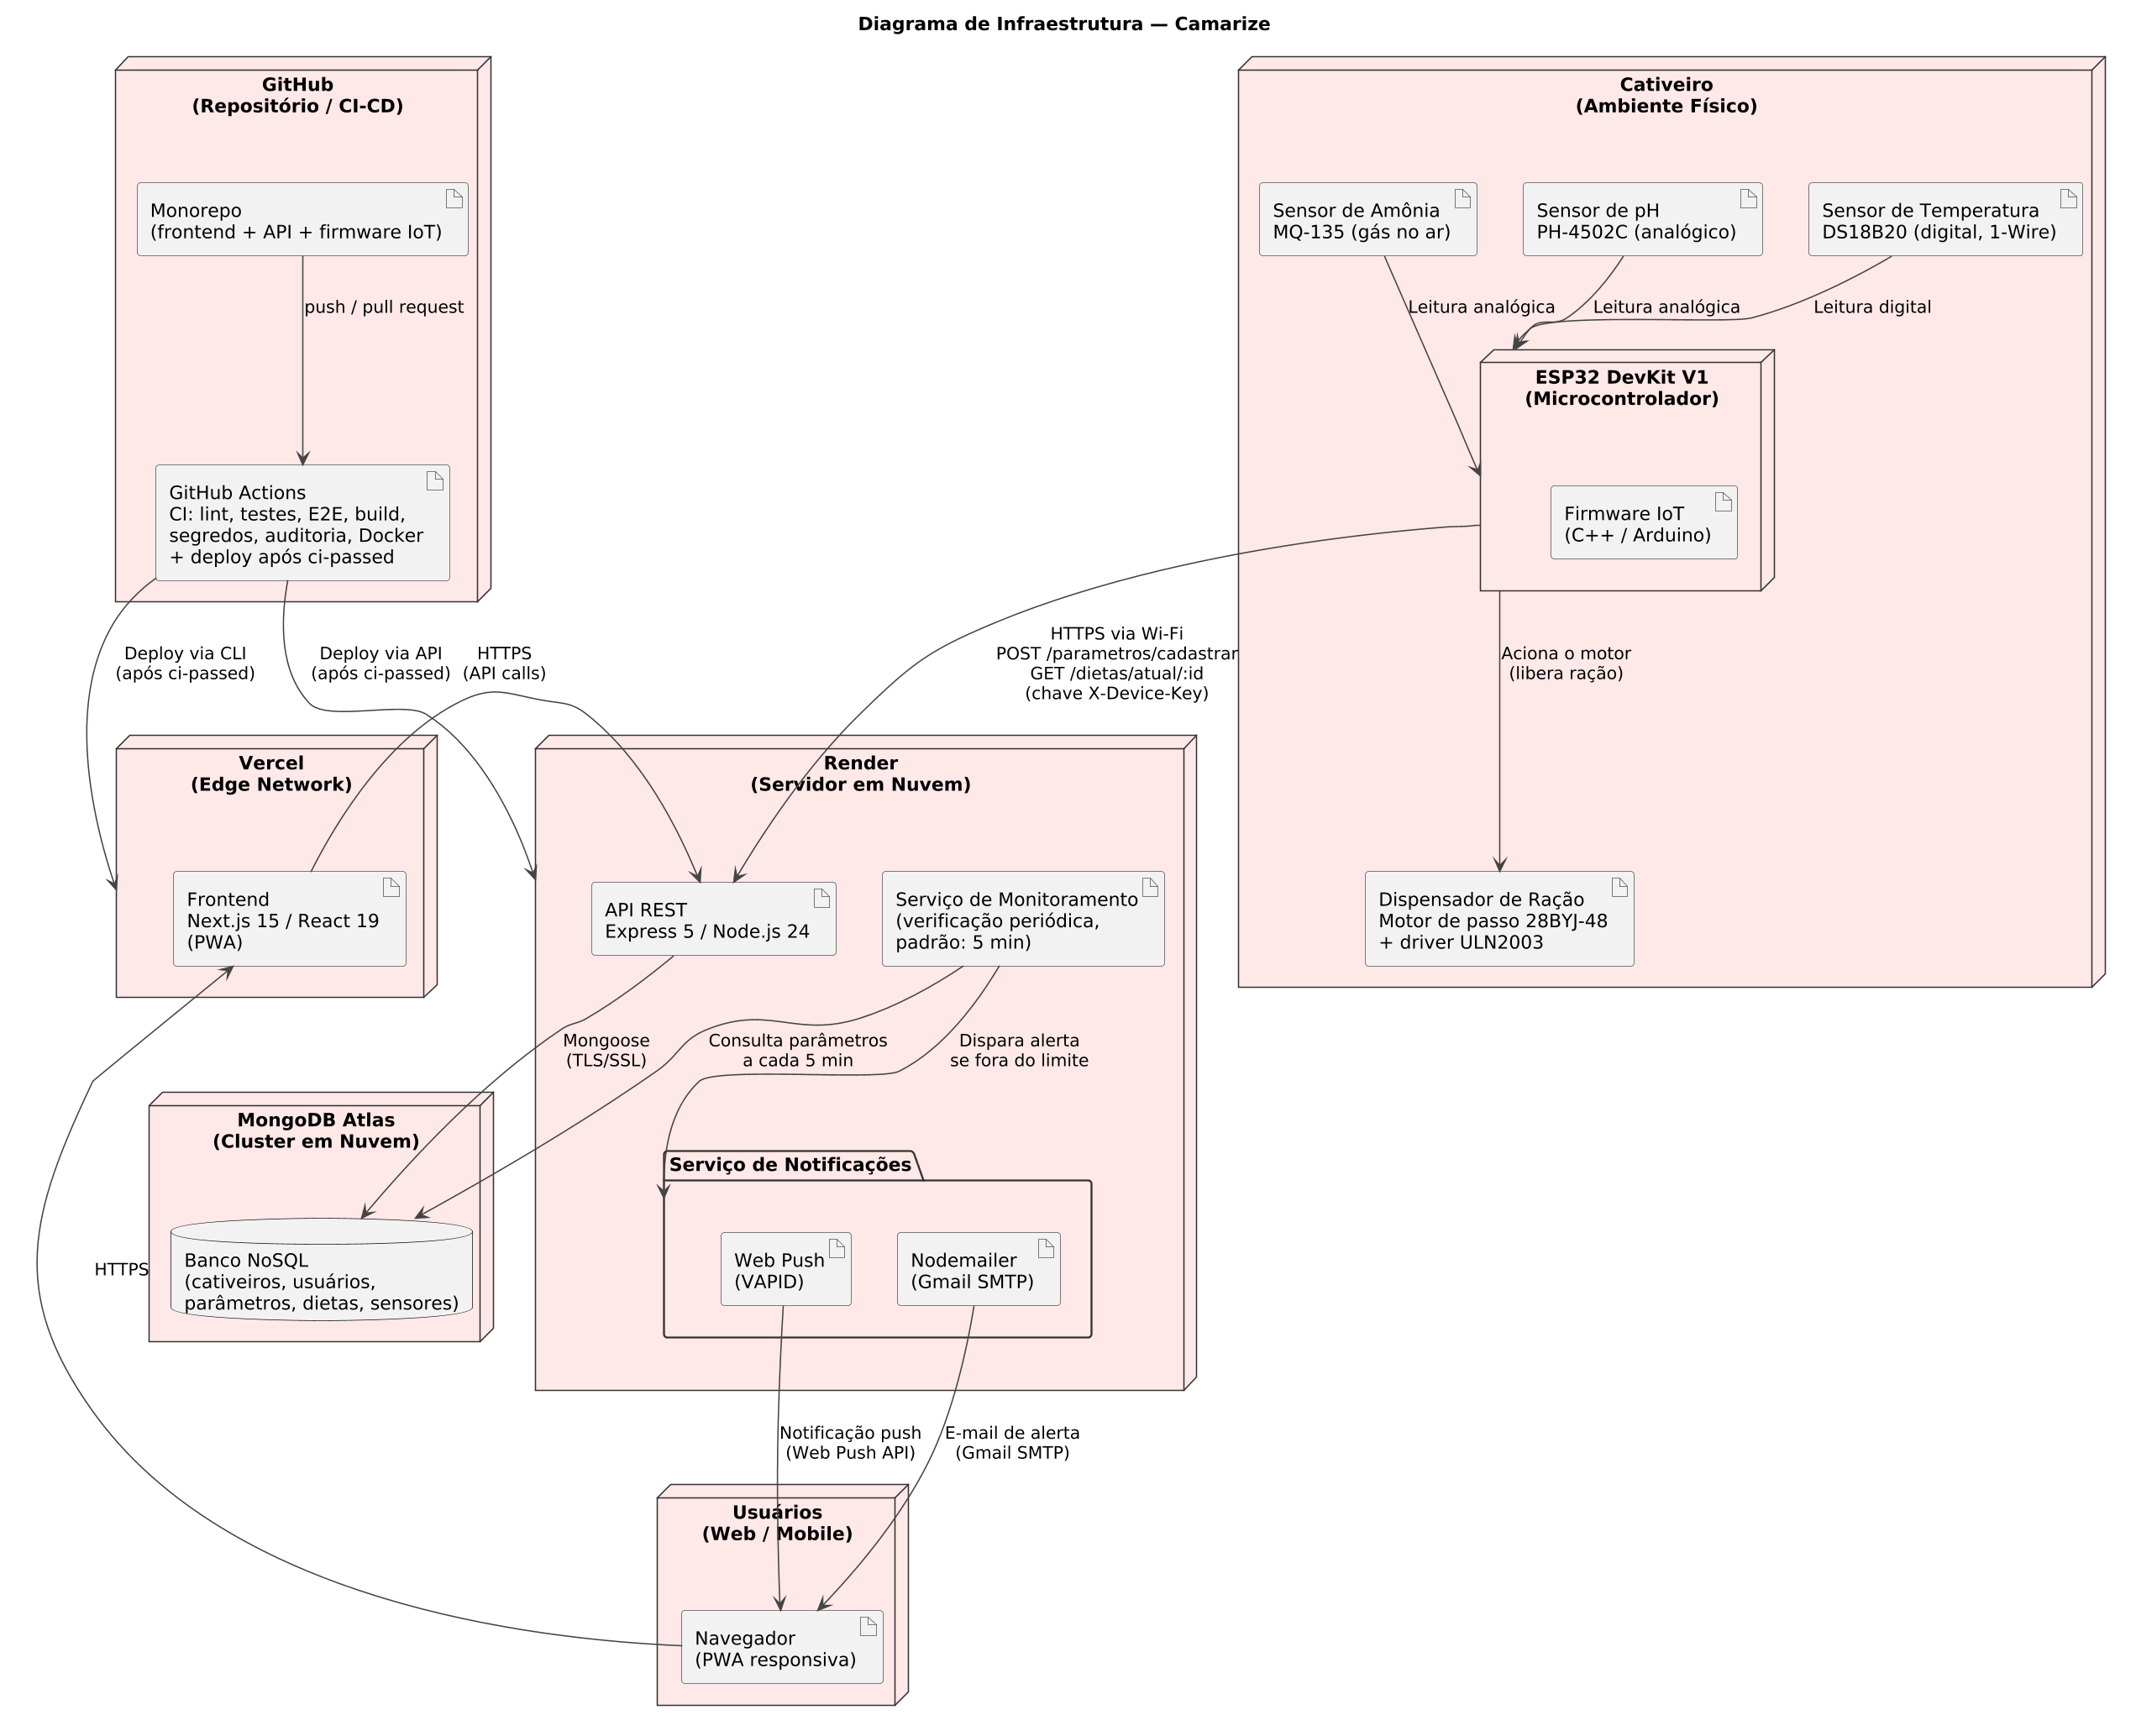
\includegraphics[width=\textwidth]{imgs/diagrama_infraestrutura.png}
\caption{Diagrama de Infraestrutura do Sistema}
\label{fig:infrastructure-diagram}
\end{figure}

\begin{itemize}
    \item \textbf{Usuários Web/Mobile:} Acessam via navegador através de HTTPS (PWA responsiva)
    \item \textbf{Frontend:} Next.js 15 hospedado na Vercel
    \item \textbf{Backend:} API Express 5 hospedada no Render (Node.js 24)
    \item \textbf{Banco de Dados:} MongoDB Atlas (cluster em nuvem)
    \item \textbf{Monitoramento:} Serviço interno com verificação periódica dos parâmetros dos cativeiros
    \item \textbf{Notificações:} Nodemailer (Gmail SMTP) para alertas por e-mail e Web Push para notificações no navegador
    \item \textbf{ESP32:} Sensores IoT enviando dados de temperatura, pH e amônia via API REST
\end{itemize}

\subsection{Arquitetura de Deploy}
A arquitetura de deployment em produção utiliza serviços gerenciados na nuvem, com a publicação feita pelo GitHub Actions:
\begin{figure}[H]
\centering
\begin{tikzpicture}[
    node distance=2cm,
    component/.style={rectangle, draw, rounded corners,
                      fill=secondarycolor!20,
                      text width=3cm,
                      align=center,
                      minimum height=1.2cm}
]
\node[component] (user) {Usuário\\(Browser/PWA)};
\node[component, below left of=user, xshift=-2cm, yshift=-1cm] (vercel) {Vercel\\(Frontend)};
\node[component, below right of=user, xshift=2cm, yshift=-1cm] (render) {Render\\(API Backend)};
\node[component, below of=render, yshift=-1.5cm] (mongo) {MongoDB Atlas\\(Banco de Dados)};
\node[component, below of=vercel, yshift=-1.5cm] (github) {GitHub Actions\\(CI e deploy)};
\draw[->, thick] (user) -- (vercel);
\draw[->, thick] (user) -- (render);
\draw[<->, thick] (vercel) -- node[above, font=\scriptsize] {API calls} (render);
\draw[<->, thick] (render) -- (mongo);
\draw[->, thick, dashed] (github) -- node[left, font=\scriptsize] {deploy via CLI} (vercel);
\draw[->, thick, dashed] (github) -- node[right, font=\scriptsize] {deploy via API} (render);
\end{tikzpicture}
\caption{Arquitetura de Deployment em Produção}
\label{fig:deployment}
\end{figure}

\subsection{Configuração Docker Compose (Desenvolvimento)}
Para o ambiente de desenvolvimento local, o arquivo \texttt{tools/docker-compose.yml} orquestra a API e o frontend. Em produção, o frontend é publicado na Vercel e a API no Render, e o CI valida o \textit{build} das imagens Docker:
\begin{verbatim}
services:
  api:
    build: ../api
    env_file: ../api/.env.docker
    environment:
      - NODE_ENV=production
      - PORT=4000
    ports:
      - "4000:4000"
  frontend:
    build:
      context: ../front-react
      target: development
    environment:
      - NEXT_PUBLIC_API_URL=http://localhost:4000
      - NEXT_PUBLIC_SSE_URL=http://localhost:4000
    depends_on:
      - api
    ports:
      - "3000:3000"
\end{verbatim} 

\subsection{Monitoramento e Alertas}
O sistema possui um serviço de monitoramento automático que verifica periodicamente os parâmetros dos cativeiros:
\begin{itemize}
    \item \textbf{Intervalo de Verificação:} Definido por variável de ambiente (\texttt{MONITORING\_\allowbreak INTERVAL\_\allowbreak MINUTES}, padrão: 5 minutos)
    \item \textbf{Parâmetros Monitorados:} Temperatura, pH e Amônia
    \item \textbf{Tolerâncias:} Temperatura (15\%), pH (20\%), Amônia (25\%)
    \item \textbf{Severidade:} Classificação automática em \texttt{media} ou \texttt{alta}
    \item \textbf{Canais de Alerta:} E-mail (Gmail SMTP via Nodemailer) com respeito a quiet hours e rate limiting
    \item \textbf{Health Check:} Endpoint \texttt{/api/health} para verificação do status da API e banco de dados
\end{itemize}

\subsection{Métricas e SLA}

As métricas a seguir são \textbf{valores de referência} publicados pelas plataformas de hospedagem utilizadas (Vercel e Render), e não medições obtidas diretamente do projeto. Servem como parâmetros de expectativa para o comportamento da infraestrutura em produção:

\begin{itemize}
    \item \textbf{Disponibilidade:} 99.9\% (SLA garantido pela Vercel e Render em seus respectivos planos)
    \item \textbf{Tempo de Resposta:} < 200ms (média estimada, favorecida pela edge network da Vercel)
    \item \textbf{Taxa de Erro:} < 0.1\% (referência da plataforma)
    \item \textbf{Throughput:} 1000 requisições/segundo (capacidade nominal da infraestrutura)
    \item \textbf{Deploy Frequency:} A cada push na branch \texttt{main} (deploy contínuo)
    \item \textbf{Lead Time:} < 1 hora (estimativa baseada no fluxo atual de desenvolvimento)
    \item \textbf{MTTR:} < 30 minutos (Mean Time To Recovery, estimativa operacional)
\end{itemize}

\newpage
\section*{Conclusão}

O conjunto de artefatos apresentado neste documento reflete o planejamento e a fundamentação técnica do projeto de monitoramento IoT para carcinicultura. A análise do Business Model Canvas, complementada pela interpretação estratégica dos nove blocos, evidenciou um modelo de negócio centrado na automação e na redução de custos operacionais para produtores de camarão. A análise SWOT identificou a dependência de conectividade e o custo inicial como principais desafios internos, contrabalançados pelo crescimento do mercado de aquicultura e pela demanda por soluções sustentáveis.

A seção de UX/UI foi estruturada com guia de estilos, tipografia, componentes visuais, persona do usuário-alvo e jornada de uso, fundamentando as decisões de \textit{design} na pesquisa de campo realizada com produtores do Vale do Ribeira.

No âmbito técnico, os sete diagramas UML documentam a arquitetura completa do sistema, desde os casos de uso até a infraestrutura de implantação, fornecendo uma visão abrangente das interações entre os componentes. A modelagem do banco de dados não relacional (MongoDB) foi detalhada nos níveis conceitual, lógico e físico, refletindo a implementação real do sistema com \textit{Mongoose Schemas}. A infraestrutura DevOps implementada, com \textit{pipeline} CI/CD via GitHub Actions, containerização com Docker para desenvolvimento local e \textit{deploy} contínuo nas plataformas Vercel e Render, garante um fluxo de entrega automatizado e rastreável.

O website institucional da equipe complementa a documentação ao padronizar a identidade visual e os canais de comunicação do projeto. Em conjunto, os artefatos formam uma base documental coerente que sustenta o desenvolvimento, a manutenção e a evolução futura do sistema.

\vspace{1cm}
\noindent\rule{\textwidth}{0.5pt}
\vspace{0.3cm}

\newpage
\addcontentsline{toc}{section}{Referências}
\bibliography{referencias}

\end{document}